\chapter{System Design and Architecture}

The system constructed for this dissertation is organised as a
five-component pipeline, shown in Figure 3.1: a shared data layer feeds
two independent generation paths --- a zero-shot baseline inference
engine and a QLoRA fine-tuning module --- the output of the fine-tuning
module is consumed by the BMAD agentic correction loop, and the outputs
of both the baseline path and the agentic loop converge on a common
evaluation and statistical analysis module that produces the comparative
results reported in Chapter 5. This chapter describes each component at
the level of its responsibilities and interfaces; the concrete
implementation of each component, including the engineering revisions
made to the agentic loop after an initial design proved unreliable, is
described in Chapter 4.

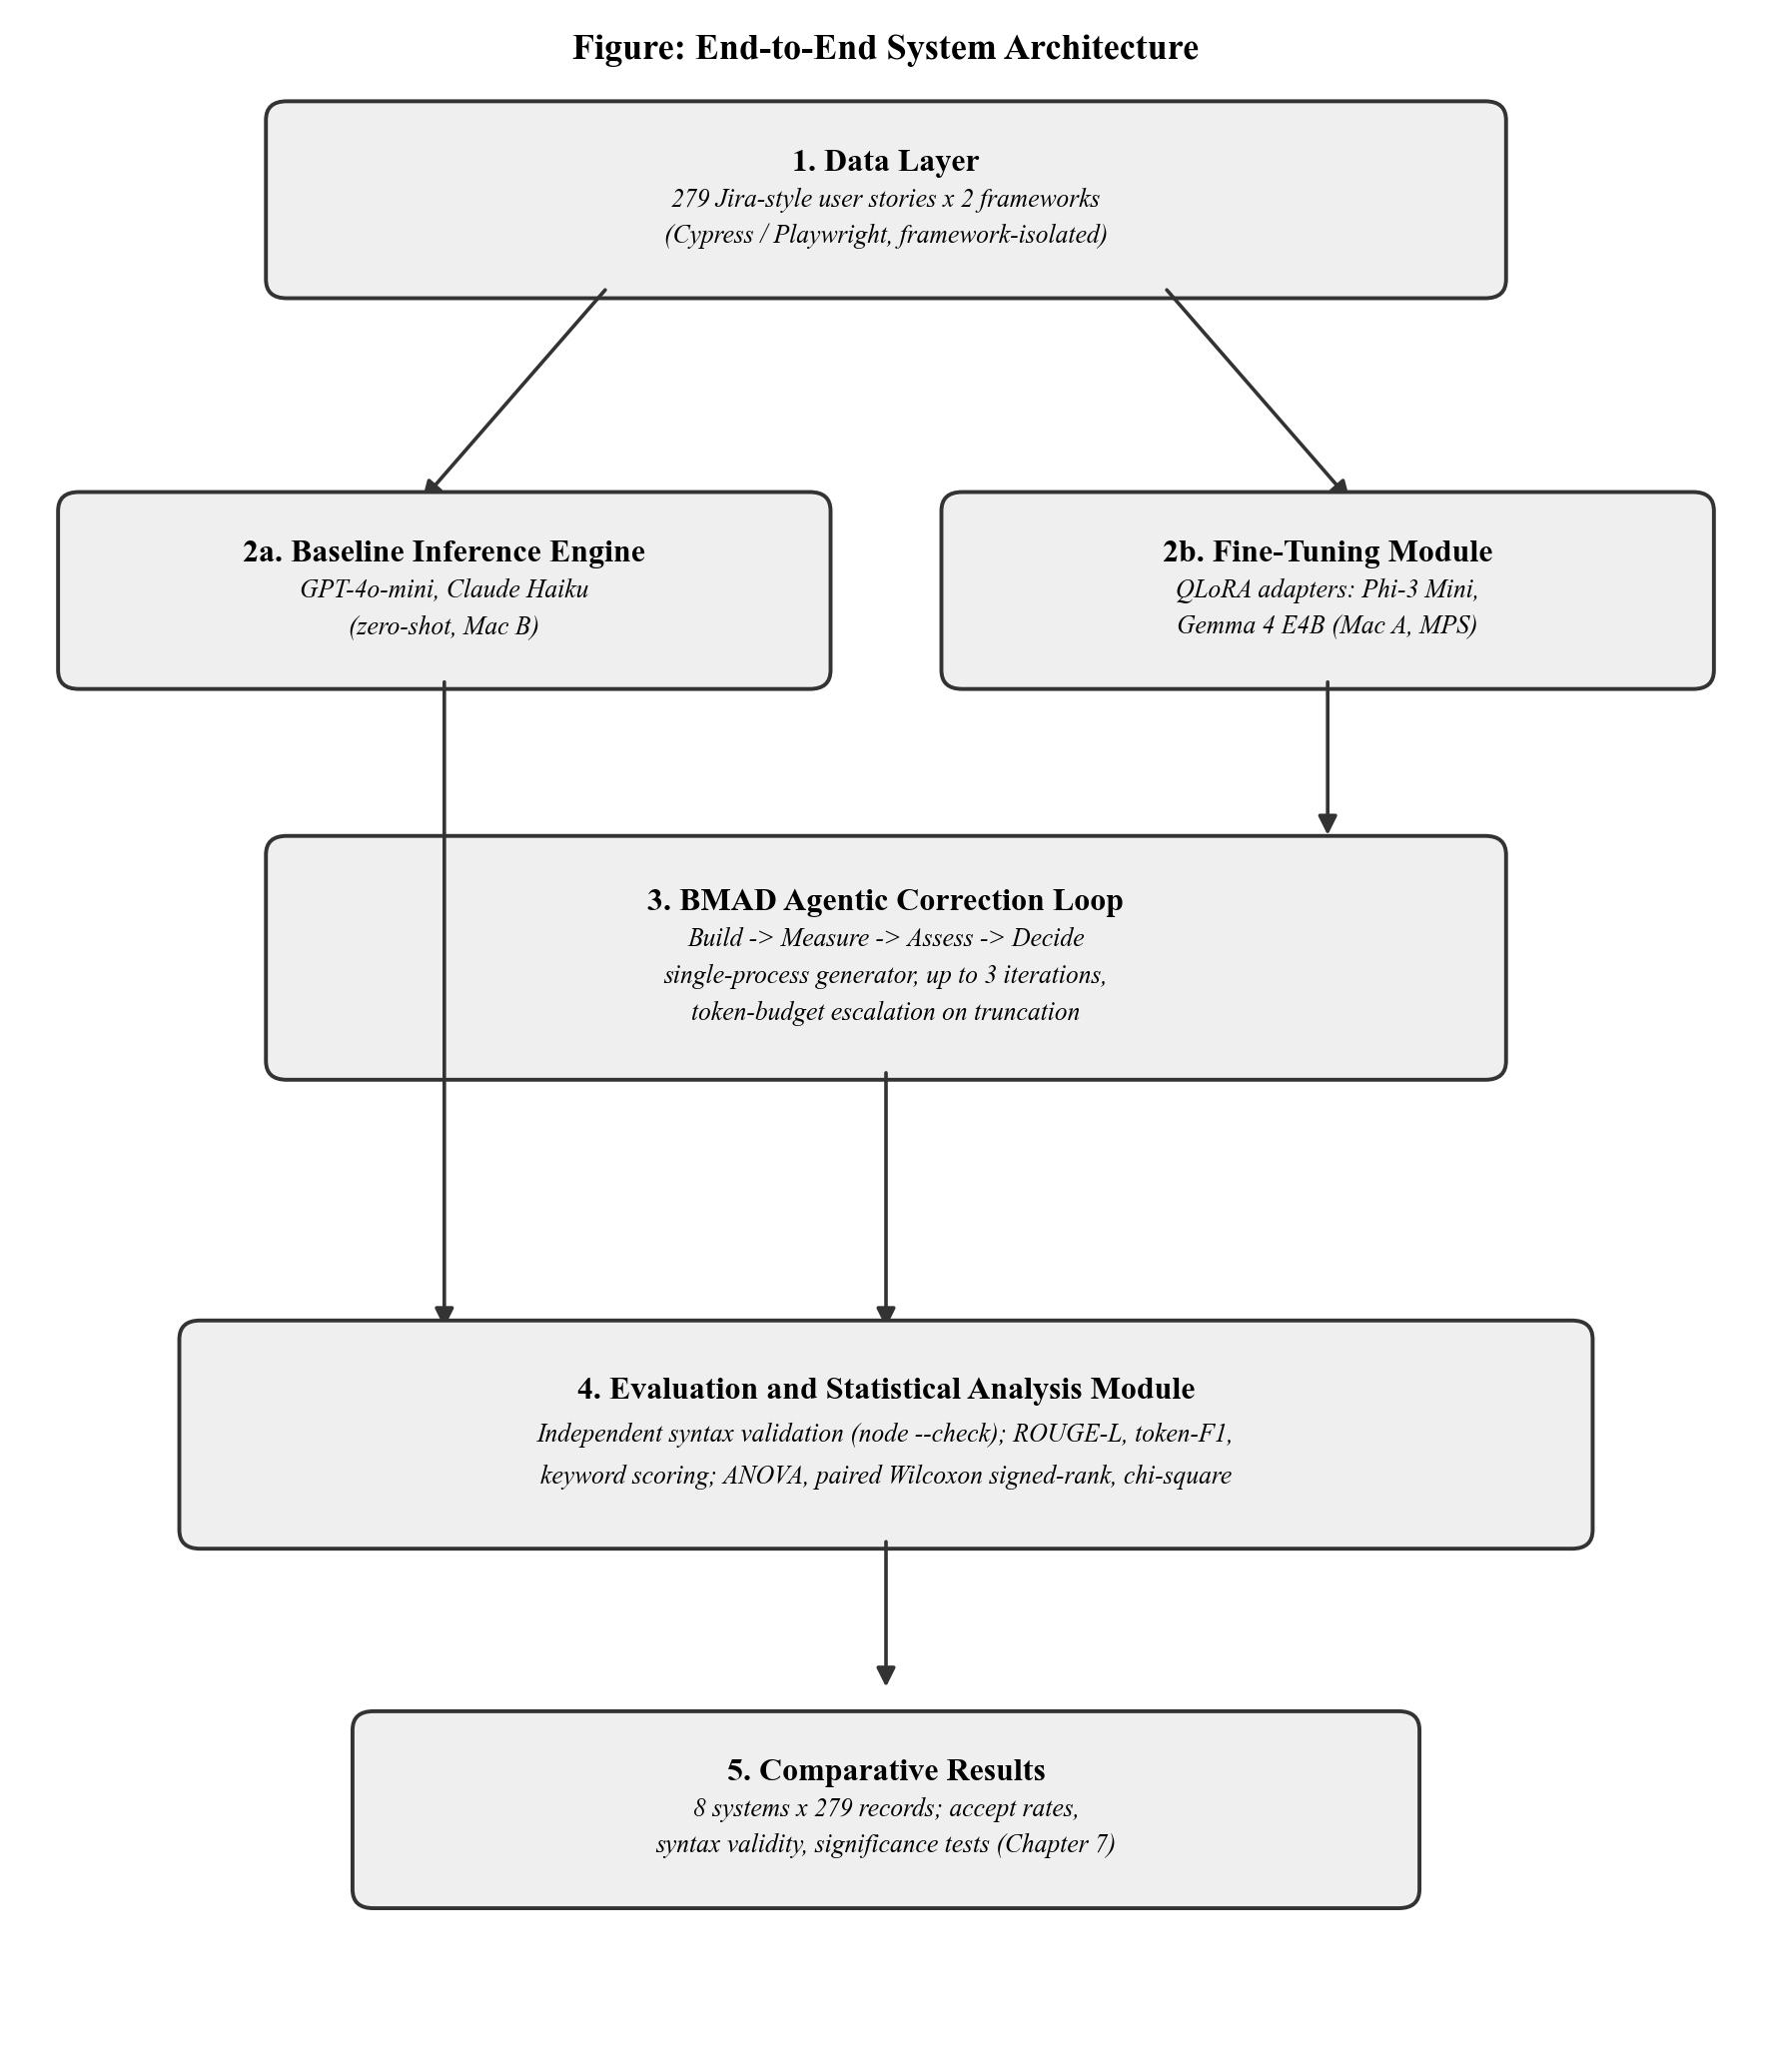
\includegraphics[width=4.47917in,height=5.26042in]{images/architecture.png}

\emph{\textbf{Figure 3.1: End-to-end system architecture}}

\section{Data Layer}

The data layer is the single source of truth consumed by every
downstream component. It comprises the 279-story dataset described in
Chapter 4, together with the two framework-isolated JSON Lines files
derived from it --- one restricted to Cypress reference scripts and one
to Playwright reference scripts. Isolating the two frameworks at the
data layer, rather than filtering by framework at consumption time,
guarantees that a fine-tuning run or a baseline inference run for one
framework has no access whatsoever to the other framework's syntax,
eliminating a class of cross-contamination that would otherwise be
possible if a single mixed-framework file were filtered downstream.

\section{Baseline Inference Engine}

The baseline inference engine routes each user story to the two
commercial large language models under evaluation --- GPT-4o-mini and
Claude Haiku --- using each provider's standard chat-completion API, and
persists the result in a schema common to both providers. This component
has no dependency on local model weights or specialised hardware, and
consequently runs on the lower-specification of the two development
machines described in Chapter 4. Architecturally, it is deliberately
independent of the fine-tuning and agentic-loop components: a baseline
result for a given story can be produced, and was in practice produced,
before the corresponding fine-tuned adapters existed.

\section{Fine-Tuning Module}

The fine-tuning module applies QLoRA adapters to two frozen open-weight
base models, Phi-3 Mini and Gemma 4 E4B, using the framework-isolated
training splits from the data layer. Each of the two models is trained
independently for each of the two frameworks, yielding four adapters in
total, each stored separately from its base model so that a given base
model can be paired with either adapter at inference time without
reloading the (much larger) base weights. This design --- one adapter
per model per framework, rather than a single adapter trained on a
mixed-framework corpus --- is the architectural mechanism by which
framework isolation, established at the data layer, is preserved through
to the trained model itself.

\section{BMAD Agentic Correction Loop}

The BMAD loop is the component responsible for turning a single
fine-tuned generation attempt into an accepted, quality-checked script.
Architecturally it implements a closed cycle of four stages applied to
each user story in turn: Build, in which the appropriate fine-tuned
adapter generates a candidate script from the user story; Measure, in
which the candidate is scored against a composite rubric combining
syntax-keyword completeness, assertion density, and similarity to a
retrieval-matched exemplar; Assess, in which that composite score is
compared against an acceptance threshold; and Decide, in which the loop
either accepts the candidate or constructs targeted corrective feedback
and returns to Build for a further attempt, bounded at three iterations
in total. This chapter treats the loop as an architectural unit with a
defined input (a user story and a target framework) and output (an
accepted or best-effort script plus its full scoring history); Chapter 4
describes how this unit is realised in code, including a significant
revision to how the Build stage communicates with the underlying model.

\section{Evaluation and Statistical Analysis Module}

The evaluation module is the only component with visibility into the
outputs of both generation paths simultaneously. It applies two
independent forms of assessment to every script produced by any of the
eight systems under study (two baseline models and two fine-tuned
models, each across two frameworks): a static syntax check using each
framework's underlying language parser, and a set of semantic-similarity
metrics computed against the corresponding held-out reference script. A
separate statistical analysis stage then consumes the per-record scores
from all eight systems, joined by the common user-story identifier
shared across the data layer, to compute the comparative significance
tests reported in Chapter 5. Positioning this module downstream of, and
architecturally independent from, both generation paths is a deliberate
design choice: it ensures that syntax validity and semantic similarity
are assessed identically and impartially regardless of which system ---
commercial baseline or fine-tuned adapter --- produced the script being
scored.

\section{Design Rationale}

Three architectural decisions recur across the components described
above and are stated explicitly here because they are foundational to
the validity of the comparison in Chapter 5. First, framework isolation
is enforced at the data layer and preserved through fine-tuning rather
than being applied only at evaluation time, so that no component in the
fine-tuned path is ever exposed to the other framework's conventions.
Second, the baseline inference engine and the fine-tuning/agentic-loop
path are architecturally independent of each other, sharing only the
common data layer and the common evaluation module; this allows either
path to be re-run, extended, or replaced without affecting the other,
and reflects the two-machine development split described in Chapter 4.
Third, evaluation is deliberately decoupled from generation: the BMAD
loop's own acceptance decision is never treated as the final word on a
script's quality, and every script --- regardless of which system
produced it --- is re-assessed by the same independent syntax and
similarity checks in the evaluation module, which is what makes the
comparison across all eight systems in Chapter 5 methodologically fair.
